%%% The main file. It contains definitions of basic parameters and includes all other parts.

%% Settings for single-side (simplex) printing
% Margins: left 40mm, right 25mm, top and bottom 25mm
% (but beware, LaTeX adds 1in implicitly)
\documentclass[12pt,a4paper]{report}
\setlength\textwidth{145mm}
\setlength\textheight{247mm}
\setlength\oddsidemargin{15mm}
\setlength\evensidemargin{15mm}
\setlength\topmargin{0mm}
\setlength\headsep{0mm}
\setlength\headheight{0mm}
% \openright makes the following text appear on a right-hand page
\let\openright=\clearpage

%% Settings for two-sided (duplex) printing
% \documentclass[12pt,a4paper,twoside,openright]{report}
% \setlength\textwidth{145mm}
% \setlength\textheight{247mm}
% \setlength\oddsidemargin{14.2mm}
% \setlength\evensidemargin{0mm}
% \setlength\topmargin{0mm}
% \setlength\headsep{0mm}
% \setlength\headheight{0mm}
% \let\openright=\cleardoublepage

%% Generate PDF/A-2u
\usepackage[a-2u]{pdfx}

%% Character encoding: usually latin2, cp1250 or utf8:
\usepackage[utf8]{inputenc}

%% Prefer Latin Modern fonts
\usepackage{lmodern}

%% Further useful packages (included in most LaTeX distributions)
\usepackage{amsmath}        % extensions for typesetting of math
\usepackage{amsfonts}       % math fonts
\usepackage{amsthm}         % theorems, definitions, etc.
\usepackage{amssymb}
\usepackage{bbding}         % various symbols (squares, asterisks, scissors, ...)
\usepackage{bm}             % boldface symbols (\bm)
\usepackage{graphicx}       % embedding of pictures
\usepackage{fancyvrb}       % improved verbatim environment
\usepackage{natbib}         % citation style AUTHOR (YEAR), or AUTHOR [NUMBER]
\usepackage[nottoc]{tocbibind} % makes sure that bibliography and the lists
			    % of figures/tables are included in the table
			    % of contents
\usepackage{dcolumn}        % improved alignment of table columns
\usepackage{booktabs}       % improved horizontal lines in tables
\usepackage{paralist}       % improved enumerate and itemize
\usepackage[usenames]{xcolor}  % typesetting in color

\usepackage{tikz}
\usetikzlibrary{automata}
\usetikzlibrary{positioning}
\usetikzlibrary{arrows}
\tikzset{my_automaton/.style={->,>=latex,semithick,bend angle=20}}
\tikzset{my_state/.style={circle, very thick, minimum size=0.4cm}}
\tikzset{my_named_state/.style={circle, thick, minimum size=0.7cm, inner sep=0.05cm}}
\tikzset{my_initial_state/.style={initial by arrow, initial text=}}
\tikzset{my_accepting_state/.style={accepting by double, thick}}

\usepackage{subfig}
\captionsetup{format=hang,margin=5pt}

\usepackage{etoolbox}

%% SPECIMEN
% Parts marked as SPECIMEN are used for building the example PDF.
% When the official template is generated by ./mkdist, all such parts
% are deleted, as well as all calls of \X and \XXX macros.
\def\X#1{\textcolor{red}{[#1]}}
\def\XXX#1{\par\smallskip\noindent \textcolor{red}{[#1]}}
%% NEMICEPS

%%% Basic information on the thesis

% Thesis title in English (exactly as in the formal assignment)
\def\ThesisTitle{Thesis title \X{as in the formal assignment}}

% Author of the thesis
\def\ThesisAuthor{Tomáš Svoboda}

% Year when the thesis is submitted
\def\YearSubmitted{2017}
\def\PlaceSubmitted{Prague}

% Name of the department or institute, where the work was officially assigned
% (according to the Organizational Structure of MFF UK in English,
% or a full name of a department outside MFF)
\def\Department{Department of Algebra}

% Is it a department (katedra), or an institute (ústav)?
\def\DeptType{Department}

% Thesis supervisor: name, surname and titles
\def\Supervisor{doc. Štěpán Holub, Ph.D.}

% Supervisor's department (again according to Organizational structure of MFF)
\def\SupervisorsDepartment{Department of Algebra}

% Study programme and specialization
\def\StudyProgramme{Mathematics}
\def\StudyBranch{Mathematical Methods of Information Security}

% An optional dedication: you can thank whomever you wish (your supervisor,
% consultant, a person who lent the software, etc.)
\def\Dedication{%
Dedication.
}

% Abstract (recommended length around 80-200 words; this is not a copy of your thesis assignment!)
\def\Abstract{%
Abstract. \X{Recommended length around 80--200 words. This is not a~copy of your thesis assignment!}
}

% 3 to 5 keywords (recommended), each enclosed in curly braces
\def\Keywords{%
{key} {words} \X{usually 3 to~5 key words or phrases}
}

%% The hyperref package for clickable links in PDF and also for storing
%% metadata to PDF (including the table of contents).
%% Most settings are pre-set by the pdfx package.
\hypersetup{unicode}
\hypersetup{breaklinks=true}

% Definitions of macros (see description inside)
%%% This file contains definitions of various useful macros and environments %%%
%%% Please add more macros here instead of cluttering other files with them. %%%

%%% Minor tweaks of style

% These macros employ a little dirty trick to convince LaTeX to typeset
% chapter headings sanely, without lots of empty space above them.
% Feel free to ignore.
\makeatletter
\def\@makechapterhead#1{
  {\parindent \z@ \raggedright \normalfont
   \Huge\bfseries \thechapter. #1
   \par\nobreak
   \vskip 20\p@
}}
\def\@makeschapterhead#1{
  {\parindent \z@ \raggedright \normalfont
   \Huge\bfseries #1
   \par\nobreak
   \vskip 20\p@
}}
\makeatother

% This macro defines a chapter, which is not numbered, but is included
% in the table of contents.
\def\chapwithtoc#1{
\chapter*{#1}
\addcontentsline{toc}{chapter}{#1}
}

% Draw black "slugs" whenever a line overflows, so that we can spot it easily.
\overfullrule=1mm

%%% Macros for definitions, theorems, claims, examples, ... (requires amsthm package)

\theoremstyle{plain}
\newtheorem{thm}{Theorem}
\newtheorem{lemma}[thm]{Lemma}
\newtheorem{claim}[thm]{Claim}

\theoremstyle{plain}
\newtheorem{defn}{Definition}

\theoremstyle{remark}
\newtheorem*{cor}{Corollary}
\newtheorem*{rem}{Remark}
\newtheorem*{example}{Example}

%%% An environment for proofs

%%% FIXME %%% \newenvironment{proof}{
%%% FIXME %%%   \par\medskip\noindent
%%% FIXME %%%   \textit{Proof}.
%%% FIXME %%% }{
%%% FIXME %%% \newline
%%% FIXME %%% \rightline{$\square$}  % or \SquareCastShadowBottomRight from bbding package
%%% FIXME %%% }

%%% An environment for typesetting of program code and input/output
%%% of programs. (Requires the fancyvrb package -- fancy verbatim.)

\DefineVerbatimEnvironment{code}{Verbatim}{fontsize=\small, frame=single}

%%% The field of all real and natural numbers
\newcommand{\R}{\mathbb{R}}
\newcommand{\N}{\mathbb{N}}

%%% Useful operators for statistics and probability
\DeclareMathOperator{\pr}{\textsf{P}}
\DeclareMathOperator{\E}{\textsf{E}\,}
\DeclareMathOperator{\var}{\textrm{var}}
\DeclareMathOperator{\sd}{\textrm{sd}}

%%% Transposition of a vector/matrix
\newcommand{\T}[1]{#1^\top}

%%% Various math goodies
\newcommand{\goto}{\rightarrow}
\newcommand{\gotop}{\stackrel{P}{\longrightarrow}}
\newcommand{\maon}[1]{o(n^{#1})}
\newcommand{\abs}[1]{\left|{#1}\right|}
\newcommand{\dint}{\int_0^\tau\!\!\int_0^\tau}
\newcommand{\isqr}[1]{\frac{1}{\sqrt{#1}}}

%%% Various table goodies
\newcommand{\pulrad}[1]{\raisebox{1.5ex}[0pt]{#1}}
\newcommand{\mc}[1]{\multicolumn{1}{c}{#1}}


% Title page and various mandatory informational pages
\begin{document}
%%% Title page of the thesis and other mandatory pages

%%% SPECIMEN
%%% Inscriptions at the opening page of the hard cover

\pagestyle{empty}
\hypersetup{pageanchor=false}
\XXX{Opening page of the hard cover. Not a part of the electronic version.}
\begin{center}

\large
Charles University

\medskip

Faculty of Mathematics and Physics

\vfill

{\huge\bf BACHELOR THESIS}

\vfill

\hbox to \hsize{\YearSubmitted\hfil \ThesisAuthor}

\end{center}

\newpage\openright

%%% NEMICEPS

%%% Title page of the thesis

\pagestyle{empty}
\hypersetup{pageanchor=false}
\begin{center}

\centerline{\mbox{
\includegraphics[width=166mm]{../img/logo-en.pdf}}}

\vspace{-8mm}
\vfill

{\bf\Large BACHELOR THESIS}

\vfill

{\LARGE\ThesisAuthor}

\vspace{15mm}

{\LARGE\bfseries\ThesisTitle}

\vfill

\Department

\vfill

\begin{tabular}{rl}

Supervisor of the bachelor thesis: & \Supervisor \\
\noalign{\vspace{2mm}}
Study programme: & \StudyProgramme \\
\noalign{\vspace{2mm}}
Study branch: & \StudyBranch \\
\end{tabular}

\vfill

% Zde doplňte rok
Prague \YearSubmitted

\end{center}

\newpage

%%% Here should be a bound sheet included -- a signed copy of the "bachelor
%%% thesis assignment". This assignment is NOT a part of the electronic
%%% version of the thesis. DO NOT SCAN.

%%% A page with a solemn declaration to the bachelor thesis

\openright
\hypersetup{pageanchor=true}
\pagestyle{plain}
\pagenumbering{roman}
\vglue 0pt plus 1fill

\noindent
I declare that I carried out this bachelor thesis independently, and only with the cited
sources, literature and other professional sources.

\medskip\noindent
I understand that my work relates to the rights and obligations under the Act No.~121/2000 Sb.,
the Copyright Act, as amended, in particular the fact that the Charles
University has the right to conclude a license agreement on the use of this
work as a school work pursuant to Section 60 subsection 1 of the Copyright Act.

\vspace{10mm}

\hbox{\hbox to 0.5\hsize{%
In ........ date ............	% FIXME!
\hss}\hbox to 0.5\hsize{%
signature of the author
\hss}}

\vspace{20mm}
\newpage

%%% Dedication

% TEMP
% \openright
% \noindent
% \Dedication
% \newpage

%%% Mandatory information page of the thesis

\openright

\vbox to 0.5\vsize{
\setlength\parindent{0mm}
\setlength\parskip{5mm}

Title:
\ThesisTitle

Author:
\ThesisAuthor

\DeptType:
\Department

Supervisor:
\Supervisor, \SupervisorsDepartment

Abstract:
\Abstract

Keywords:
\Keywords

\vss}

\newpage

\openright
\pagestyle{plain}
\pagenumbering{arabic}
\setcounter{page}{1}


%%% A page with automatically generated table of contents of the bachelor thesis

\tableofcontents

%%% Each chapter is kept in a separate file
%\chapter*{Introduction}
\addcontentsline{toc}{chapter}{Introduction}


\chapter{Eggan's question}

\cite{Eggan63} asks whether there are languages with arbitrarily large star height. In this section we present proof first due to~\cite{DejeanSchutzenberger66} and recently formulated in~\cite{Sakarovitch09}.

Throughout this chapter we use language $W_q = {\{f \mid |f|_a \equiv |f|_b \bmod 2^q \}}$.

\begin{lemma}
    For language~$W_q$ there is an expression of star height~$q$, that denotes~$W_q$.
\end{lemma}

\begin{proof}
    $W_q$ is recognised by an automaton~${\mathcal{R}(2^q)}$. By following a specific order~$\omega$ in the elimination method on $W_q$ we get an expression of a~star height $q$. First we set expressions
    \begin{alignat*}{5}
        X_1 = a^2 , \quad Y_1 = b^2, \quad &\text{ and } \quad Z_1 = ab + ba.
    \intertext{Then for every integer $n$ we have}
        X_{n+1} = X_n Z_n^* X_n , \quad Y_{n+1} = Y_n Z_n^* Y_n, \quad &\text{ and } \quad Z_{n+1} = Z_n + X_n Z_n^* Y_n + Y_n Z_n^* X_n.
    \end{alignat*}
    It follows that
    \[
        W_q = {(X_q + Y_q + Z_q)}^*.
    \]
    Since $X_n , Y_n , \text{ and } Z_n$ have star height~$n~-~1$, we have got an expression denoting~$W_q$ of star height~$q$.
\end{proof}

\begin{figure}[h]
    \centering
        \begin{tikzpicture}[my_automaton]
    \tikzstyle{every state}=[my_state]
    \tikzstyle{initial}=[my_initial_state]
    \tikzstyle{accepting}=[my_accepting_state]
    %\draw[help lines] (-1.5,1.5) grid (1.5,-1.5);
    \node[state, initial, accepting] (0) at (180:1.5) {};
    \node[state] (1) at (135:1.5) {};
    \node[state] (2) at (90:1.5) {};
    \node[state] (3) at (45:1.5) {};
    \node[state] (4) at (0:1.5) {};
    \node[state] (5) at (-45:1.5) {};
    \node[state] (6) at (-90:1.5) {};
    \node[state] (7) at (-135:1.5) {};

    \path
        (0) edge [bend left] node [near start, above left=-1mm] {$a$} (1)
        (1) edge [bend left] node [right] {$b$} (0)
        (1) edge [bend left] node [above] {$a$} (2)
        (2) edge [bend left] node [below right=-1mm] {$b$} (1)
        (2) edge [bend left] node [above right=-1mm] {$a$} (3)
        (3) edge [bend left] node [near start, below left=-1mm] {$b$} (2)
        (3) edge [bend left] node [right] {$a$} (4)
        (4) edge [bend left] node [left] {$b$} (3)
        (4) edge [bend left] node [right] {$a$} (5)
        (5) edge [bend left] node [above left=-1mm] {$b$} (4)
        (5) edge [bend left] node [below] {$a$} (6)
        (6) edge [bend left] node [above] {$b$} (5)
        (6) edge [bend left] node [below] {$a$} (7)
        (7) edge [bend left] node [above] {$b$} (6)
        (7) edge [bend left] node [left] {$a$} (0)
        (0) edge [bend left] node [above right=-1mm] {$b$} (7)
    ;
\end{tikzpicture}
    \caption{Automaton~${\mathcal{R}(8)}$}\label{fig:automaton_R8}
\end{figure}

\begin{thm}\label{thm:main}
    The language $W_q = {\{f \mid |f|_a \equiv |f|_b \bmod 2^q \}}$ over ${\{a, b\}}^*$ has star height~$q$.
\end{thm}

\begin{proof}[Proof of \autoref*{thm:main}]
\end{proof}

\section{Title of the first subchapter of the first chapter}
\chapter{Eggan's question}

\cite{Eggan63} asks whether there are languages with arbitrarily large star height. In this section we present proof first due to~\cite{DejeanSchutzenberger66} and recently formulated in~\cite{Sakarovitch09}.

Throughout this chapter we use language $W_q = {\{f \mid |f|_a \equiv |f|_b \bmod 2^q \}}$.

\begin{lemma}
    For language~$W_q$ there is an expression of star height~$q$, that denotes~$W_q$.
\end{lemma}

\begin{proof}
    $W_q$ is recognised by an automaton~${\mathcal{R}(2^q)}$. By following a specific order~$\omega$ in the elimination method on $W_q$ we get an expression of a~star height $q$. First we set expressions
    \begin{alignat*}{5}
        X_1 = a^2 , \quad Y_1 = b^2, \quad &\text{ and } \quad Z_1 = ab + ba.
    \intertext{Then for every integer $n$ we have}
        X_{n+1} = X_n Z_n^* X_n , \quad Y_{n+1} = Y_n Z_n^* Y_n, \quad &\text{ and } \quad Z_{n+1} = Z_n + X_n Z_n^* Y_n + Y_n Z_n^* X_n.
    \end{alignat*}
    It follows that
    \[
        W_q = {(X_q + Y_q + Z_q)}^*.
    \]
    Since $X_n , Y_n , \text{ and } Z_n$ have star height~$n~-~1$, we have got an expression denoting~$W_q$ of star height~$q$.
\end{proof}

\begin{figure}[h]
    \centering
        \begin{tikzpicture}[my_automaton]
    \tikzstyle{every state}=[my_state]
    \tikzstyle{initial}=[my_initial_state]
    \tikzstyle{accepting}=[my_accepting_state]
    %\draw[help lines] (-1.5,1.5) grid (1.5,-1.5);
    \node[state, initial, accepting] (0) at (180:1.5) {};
    \node[state] (1) at (135:1.5) {};
    \node[state] (2) at (90:1.5) {};
    \node[state] (3) at (45:1.5) {};
    \node[state] (4) at (0:1.5) {};
    \node[state] (5) at (-45:1.5) {};
    \node[state] (6) at (-90:1.5) {};
    \node[state] (7) at (-135:1.5) {};

    \path
        (0) edge [bend left] node [near start, above left=-1mm] {$a$} (1)
        (1) edge [bend left] node [right] {$b$} (0)
        (1) edge [bend left] node [above] {$a$} (2)
        (2) edge [bend left] node [below right=-1mm] {$b$} (1)
        (2) edge [bend left] node [above right=-1mm] {$a$} (3)
        (3) edge [bend left] node [near start, below left=-1mm] {$b$} (2)
        (3) edge [bend left] node [right] {$a$} (4)
        (4) edge [bend left] node [left] {$b$} (3)
        (4) edge [bend left] node [right] {$a$} (5)
        (5) edge [bend left] node [above left=-1mm] {$b$} (4)
        (5) edge [bend left] node [below] {$a$} (6)
        (6) edge [bend left] node [above] {$b$} (5)
        (6) edge [bend left] node [below] {$a$} (7)
        (7) edge [bend left] node [above] {$b$} (6)
        (7) edge [bend left] node [left] {$a$} (0)
        (0) edge [bend left] node [above right=-1mm] {$b$} (7)
    ;
\end{tikzpicture}
    \caption{Automaton~${\mathcal{R}(8)}$}\label{fig:automaton_R8}
\end{figure}

\begin{thm}\label{thm:main}
    The language $W_q = {\{f \mid |f|_a \equiv |f|_b \bmod 2^q \}}$ over ${\{a, b\}}^*$ has star height~$q$.
\end{thm}

\begin{proof}[Proof of \autoref*{thm:main}]
\end{proof}

\section{Title of the first subchapter of the first chapter}
\chapter{Generalisation}

The definition of star height can be expanded into \emph{generalised star height}, a~concept that is quite similar, yet current understanding of its properties is much more limited.

\section{Generalised star height}

\begin{defn}
    \emph{A generalised rational expression over $A$} is a formula obtained inductively from the letters of $A$ and the symbols $\{ \: \re{0} \: , \: \re{1} \: , \: + \: , \: \cdot \: , * \: , \: - \: , \: \wedge \: , \: ^{\prime} \: \}$ by the following process:
    \begin{itemize}
        \item[(i)] $\re{0}, \re{1}$, and $a$, for $a$ in $A$, are generalised rational expressions,
        \item[(ii)] if $\re{E}$ and $\re{F}$ are generalised rational expressions, then
            \[
                (\re{E} + \re{F}) \; , \quad (\re{E} \cdot \re{F}) \; , \quad (\re{E}^*) \; , \quad (\re{E} - \re{F}) \; , \quad (\re{E} \wedge \re{F}) \; , \quad (\re{E}^{\prime})
            \]
             are generalised rational expressions.
    \end{itemize}
    We write $\re{GRatE} A^*$ for the set of generalised rational expressions over $A$.
\end{defn}

The languages denoted by generalised rational expressions are the same as for the rational expressions plus, to accommodate the added symbols, we let:
\[
    L[\re{E} - \re{F}] = L[\re{E}] \setminus L[\re{F}] \; , \quad L[\re{E} \wedge \re{F}] = L[\re{E}] \cap L[\re{E}] \; , \quad L[\re{E}^{\prime}] = \complement_{A^*} L[\re{E}].
\]

\begin{defn}
    Let $\re{E} \in \re{GRatE} A^*$. \emph{Generalised star height} is, by induction on the complexity of expressions:
    \begin{align*}
        &\text{if } \re{E} = \re{0}, \; \re{E} = \re{1} \; \text{ or } \; \re{E} = a, \text{ for } a \in A \; , & &\gh{\re{E}} = 0 \; , \\
        &\text{if } \re{E} = \re{F} + \re{G} \; \text{ or } \; \re{E} = \re{F} \cdot \re{G}\; , & &\gh{\re{E}} = \max{(\gh{\re{F}}, \gh{\re{G}})} \; , \\
        &\text{if } \re{E} = \re{F}^* \; , & &\gh{\re{E}} = 1 + \gh{\re{F}} \; , \\
        &\text{if } \re{F} = \re{E}^{\prime} \; , & &\gh{\re{E}} = \gh{\re{F}} \; .
    \end{align*}
\end{defn}
For $\re{E} = \re{F} - \re{G}$, or $\re{E} = \re{F} \wedge \re{G}$, due to De Morgan's laws, identities exist:
\[
    \re{F} - \re{G} \equiv \re{F} \wedge \re{G}^{\prime} \; , \quad \text{and} \quad \re{F} \wedge \re{G} \equiv {(\re{F}^{\prime} + \re{G}^{\prime})}^{\prime} \;
\]
thus $\gh{\re{E}} = \max{(\gh{\re{F}}, \gh{\re{G}})}$. The generalised star height of rational language $L$ over $A^*$, written $\gh{L}$, is the minimum of the generalised star heights of the generalised rational expressions that denote $L$:
\[
    \gh{L} = \min \{ \gh{\re{E}} \mid \re{E} \in \re{GRatE} A^*: L = L[\re{E}] \} \; .
\]

\section{Open questions}

The determination of the star height of a~rational language, however a~difficult problem, has been solved. The determination of the generalised star height still remains to be solved. Two open questions, that are raised by the definition of generalised star height of rational language, are namely the existence of an~infinite hierarchy and the computation of generalised star height.

Not only do we not know whether there are rational languages with arbitrarily large generalised star height, but even language with generalised star height greater than 1 has not yet been shown. On the other hand, for languages whose generalised star height is equal to 0, or so called \emph{star-free languages}, Schützenberger~\cite{Schutzenberger65} provided an algebraic characterization.

%\chapter*{Conclusion}
\addcontentsline{toc}{chapter}{Conclusion}


%%% Bibliography
%%% Bibliography (literature used as a source)
%%%
%%% We employ bibTeX to construct the bibliography. It processes
%%% citations in the text (e.g., the \cite{...} macro) and looks up
%%% relevant entries in the bibliography.bib file.
%%%
%%% The \bibliographystyle command selects, which style will be used
%%% for references from the text. The argument in curly brackets is
%%% the name of the corresponding style file (*.bst). Both styles
%%% mentioned in this template are included in LaTeX distributions.

% \bibliographystyle{plainnat}    %% Author (year)
\bibliographystyle{unsrt}     %% [number]

\renewcommand{\bibname}{Bibliography}

%%% Generate the bibliography. Beware that if you cited no works,
%%% the empty list will be omitted completely.

\bibliography{bibliography}

%%% If case you prefer to write the bibliography manually (without bibTeX),
%%% you can use the following. Please follow the ISO 690 standard and
%%% citation conventions of your field of research.

% \begin{thebibliography}{99}
%
% \bibitem{lamport94}
%   {\sc Lamport,} Leslie.
%   \emph{\LaTeX: A Document Preparation System}.
%   2nd edition.
%   Massachusetts: Addison Wesley, 1994.
%   ISBN 0-201-52983-1.
%
% \end{thebibliography}


%%% Figures used in the thesis (consider if this is needed)
%\listoffigures

%%% Tables used in the thesis (consider if this is needed)
%%% In mathematical theses, it could be better to move the list of tables to the beginning of the thesis.
%\listoftables
%\XXX{In mathematical theses, it could be better to move the list of tables to the beginning of the thesis.}

%%% Abbreviations used in the thesis, if any, including their explanation
%%% In mathematical theses, it could be better to move the list of abbreviations to the beginning of the thesis.
%\chapwithtoc{List of Abbreviations}
%\XXX{In mathematical theses, it could be better to move the list of abbreviations to the beginning of the thesis.}

%%% Attachments to the bachelor thesis, if any. Each attachment must be
%%% referred to at least once from the text of the thesis. Attachments
%%% are numbered.
%%%
%%% The printed version should preferably contain attachments, which can be
%%% read (additional tables and charts, supplementary text, examples of
%%% program output, etc.). The electronic version is more suited for attachments
%%% which will likely be used in an electronic form rather than read (program
%%% source code, data files, interactive charts, etc.). Electronic attachments
%%% should be uploaded to SIS and optionally also included in the thesis on a~CD/DVD.
%%% Allowed file formats are specified in provision of the rector no. 13/2017.
%\appendix
%\chapter{Attachments}
%\XXX{Attachments to the bachelor thesis, if any. Each attachment must be referred to at least once from the text of the thesis. Attachments are numbered.}
%\XXX{The printed version should preferably contain attachments, which can be read (additional tables and charts, supplementary text, examples of program output, etc.). The electronic version is more suited for attachments which will likely be used in an electronic form rather than read (program source code, data files, interactive charts, etc.). Electronic attachments should be uploaded to SIS and optionally also included in the thesis on a~CD/DVD. Allowed file formats are specified in provision of the rector no. 13/2017.}

%\section{First Attachment}

\openright
\end{document}
